\documentclass[a4paper, 12pt, twoside, openright]{article}
\usepackage{t1enc}
\usepackage[utf8]{inputenc}
\usepackage{graphicx}
\usepackage{tikzsymbols} %ikonokhoz
\usepackage{hyperref}
\hypersetup{
	colorlinks,
    citecolor=black,
    filecolor=black,
    linkcolor=black,
    urlcolor=black
}
%hivatkozások feketék legyenek
\usepackage{url}
\def\UrlBreaks{\do\/\do-}
%megtörheti az urleket a / és a - karaktereknél
\usepackage{sidecap}
\usepackage{wrapfig}
\usepackage{upgreek}
%\usepackage{glossaries}
\sloppy
\frenchspacing
\usepackage[inner=1.5cm,outer=1.5cm]{geometry}
%\geometry{margin=2.5cm}

\usepackage{textcomp} %~ hullám miatt
\usepackage{float} %ábrákhoz
\usepackage{pdfpages}
\newcommand{\tab}{\hspace*{1em}}
\renewcommand*{\thefootnote}{(\arabic{footnote})}

\begin{document}

\title{Ifis játékok}
\maketitle

\begin{itemize}
\item \textbf{Hurkapálcás:} Párokban játsszuk. Minden párnak kell két hurkapálca. Egymással szemben állnak. Mutatóujjaikat felfelé tartják és a legelső ujjperceik közé beszorítanak 1-1 hurkapálcát. Nem a saját két kezük közé, hanem az egyik ember jobb kezének mutatóujja és a másik bal kezének mutatóujja tart egy hurkapálcát. A játék célja, hogy ne essen le vagy törjön el egyik hurkapálca sem. Ha minden pár felállt, akkor indulhat a játék, akinek akár az egyik hurkapálca leesik, az a pár kiesik. nem lehet a hurkapálcát megfogni, csak mutatóujjal lehet tartani. A játék indulása után a többi párt lökdösni kell, hogy elejtsék a hurkapálcát. Csípővel, vállal, könyökkel lehet lökdösni a másikat vagy annak hurkapálcáját, de fokozottan figyelni kell, hogy vigyázzunk egymásra. Az utolsó pár nyer.

\item \textbf{Családos:} Létszámtól függ, hogy egy család 3 (apa, anya, fiú) vagy 4 tagú (apa, anya, fiú, lány). Papírokat előre el kell készíteni, amire a család vezetékneve és a családtag szerepe van írva. (pl.: \emph{Takács apa} vagy \emph{Szakács lány}). Hasonló vezetékneveket kell kitalálni (Takács, Makács, Bakács, Szakács, Lakás, ...). A játék előtt kiteszünk egy nagyobb körbe annyi széket ahány család van és mindenki kap egy papírt, amit még nem nézhet meg. Ahogy indul a játék meg lehet nézni a nevet és a cél, hogy egy széken egy család legyen úgy, hogy az apa ül a széken a térdén az anya, aztán a fiú (majd a lány). Ezt úgy érik el, hogy mindenki üvöltözni kezd, hogy ki hiányzik az ő családjából (az apa célszerűen már le is ül és úgy kiabál). Amelyik család utolsónak ül le annak minden tagja kiesik. A többiek mind odaadják a papírjukat a játékvezetőnek, aki újra kiosztja azokat és kezdődhet a következő kör. Az utolsó család tagjai nyernek.
(Értelemszerűen minden körben új családhoz tartozik egy ember. Vagy 3 vagy 4 tagú családokkal játsszuk, egy játékon belül ne keverjük.)

\item \textbf{Kő, papír, olló két csoportban:} Két csoportra osztjuk a csapatot és a pályát keresztbe kettéválasztjuk egy -- képzeletbeli -- vonallal. Legalább akkora pálya kell, hogy a csapatok mögött legyen 4-5 méter a pálya végéig. Mindekettő cspat megbeszél maguk között egyet a kő-papír-olló kézmozdulatai közül, majd felsorakoznak a vonal két oldalára egymással szemben. A játékvezető jelére elhangzik a ``kő-papír-olló'' és mindkettő cspat mutatja a saját jelét. Amelyik csapat jele üti a másikét annak a csapatnak meg kell fogni a másik csapat tagjait, mielőtt azok visszafutnának a saját alapvonalukig. Akit elkapnak előtt az átáll a másik csapatba és új kör kezdődik. Aki visszajut az alapvonalig, az marad azon az oldalon a következő körig. Ha valamelyik oldal elfogy, akkor a másik csapat nyer.

\item \textbf{Ülj le az üres székre, a többi akadályozza meg:} A teremben össze-vissza szét vannak szórva székek, annyi ahányan játszanak. Egy ember nem ül széne, a többiek igen. Az álló embernek a célja, hogy leüljön az üres székre, de nem futhat. A többiek ezt úgy tudják megakadályozni, hogy mielőtt leülne a saját helyükről felállva átülnek az üres székre. Ilyenkor az álló ember célja az újonnan üreséé vált székre való leülés. Akik ülnek, azok futhatnak a székek között. Ha valaki felállt egy székről, akkor nem ülhet vissza ugyanoda. Ha az álló embernek sikerül leülnie, akkor aki helyére leült, az lesz a következő álló ember.

\item \textbf{Pénzfeldobós, kézszorítós:} Két csoportra osztjuk az embereket és van egy játékvezető. A csoportok beállnak egymással párhuzamosan két sorba, úgy hogy minden ember háttal áll a másik csapatnak. A sor egyik végén van a játékvezető és egy pénzérme a kezében a másik végén egy széken egy könnyen elvehető tárgy, például egy műanyag pohár. A pohárnak ugyanolyan távol kell lennie a két utolsó embertől. A sorban álló emberek megfogják egymás kezét. A játékvezető feldobja a pénzérmét és a kezére csapja, majd megmutatja a két első játékosnak a sorban. Ha fej van a pénzérmén, akkor mindkettő első játékos megszorítja a saját csapatában álló második játékos kezét, aki továbbszorít és így végigmegy a szorítás mindkét soron. Amikor az utolsó emberhez ér a szorítás, az felkapja a poharat. Amelyik csapat hamarabb fogta meg a poharat az kapja a pontot és a poharat megfogó játékos előrejöhet a sor elejére. Ha valami miatt tévesen kapta fel a játékos a poharat (pl. valaki tévesen szorított), akkor a tévesztő csapatból az első játékos megy a sor végére. A játék célja, hogy az egész csapat körbeforogjon (a jó irányba) és az első játékosuk újra az első helyen legyen. A játékvezető minden pénzfeldobás után várjon pár másodpercet mire újat dob, így nem egyértelmű, hogy milyet dobott előbb. Minden játékosnak kifelé kell néznie, legfőképpen nem szabad a másik csapatot és azok kezét nézni. A pénzérme jól látható legyen mindkettő első ember számára. Amikor cserélődik az első ember, célszerű megmutatni, hogy a pénzérmének melyik fele a fej.

\item \textbf{Kapd el a párod:} Két ugyanakkora létszámú csoport. Mindkettő csoport tagjai beszámozva egytől a csoportlétszámig. Kettő vonalat kell húznunk (min 5-6 méterre egymástól), amin kívül feláll két oldalt a két csapat. A pálya közepére egy tárgyat kell tenni (pl. palack, babzsák). A játékvezető mond egy számot, mindkettő csapatból az adott számú játékos célja, hogy vagy megszerezze a tárgyat és visszafusson vele a saját alapvonalára vagy megfogja a másik játékost, miközben annál van a tárgy. Ahogy a szám elhangzott befuthat a két játékos. Nem érhetnek egymáshoz csak ha valamelyik már megérintette a tárgyat. Amelyik játékos hozzárt a tárgyhoz, az olyan mintha a kezében lenne, tehát ha csak egy ujjal is hozáér, a másik játékos már megfoghatja. Ha megfogja, akkor a fogóé a pont; ha viszont a tárgyat megfogónak sikerül visszafutnia az alapvonalához, mielőtt a másik játékos megérintené, akkor az ővé a pont. A játék elején tisztázni kell, hogy teljes testtel vissza kell érni az alapvonal mögé vagy elég, ha valamelyik testrész már éri a vonalat (helytől függ, hogy melyik a jobb megoldás).

\item \textbf{Kézcsapkodós:} Körben leülnek az emberek egy asztalhoz és mindenki beteszi a kezét az asztalra, úgy hogy a mellette levővel keresztezze a kezét, tehát az én bal kezemtől jobbra van a tőlem balra ülő jobb keze, aztán attól jobbra a tőlem jobbra ülő bal keze, majd utána jobbra az én jobb kezem. Így formálunk egy kört. A játék során egy ``jel'' megy körbe. Valaki elkezdi egy tapsolásal az asztalon, a tőle jobbra levő kéz a következő, szintén egy csapással és így megy körbe a csapás. Ha valamelyik soron következő kéz duplát casp, akkor megfordul az irány és az előtte csapott kéz jön. Ha valaki rosszkor csap, annak a rosszul csapó keze kiesik. Rossz csapás, ha nem az a kéz következik; ha több mint 2 másodpercig vár vagy ha nem egyet vagy kettő csap. A csapásoknak gyorsaknak, hallhatóaknak kell lennie és egyértelműen meg kell tudni különböztetni az egy csapást a kettőtől. Aki felemeli a tenyerét az már csapásnak a számít. Minden nyugalomban levő tenyér (tehát, aki épp nem csap), az asztalon kell, hogy legyen. Amelyik két kéz marad utoljára az nyert. Ha valakinek a két keze még játszik, de mindkettő kéz kiesett közüle, akkor ugyanúgy megy tovább a játék, neki a két keze egymás mellé került.

\item \textbf{Üsd a jobboldalit:} Körben ül a társaság, eggyel több szék van, mint ahány játékos. A játék indulásakor beszámozzuk az embereket és mindenkinek az lesz a száma a játék végéig. Az emberek úgy ülnek a széken, hogy ajobb kezük a jobb térdükön van és a bal térdük szabad. Amelyik játékostól jobbra van az üres szék, az hív egy számot. Akinek a számát hívta, annak az a célja, hogy felálljob és átüljön az üres székre a hívó mellé. Aki a hívott számtól balra van (tehát akitől jobbra van, akit hívtak, innen a játék neve), az megpróbálja megakadályozni, úgy hogy mielőtt felállna a hívott játékos a jobb kezével annak a combjára csap. Ha még nem állt fel ez idő alatt a hívott játékos, akkor ott kell maradnia, mert lecsapták. Akármeddig játszható, nincs egy konkrét végkimenet. Ha a hívó játékos véletlenül a saját számát hívja vagy azt aki tőle kettővel jobbra van (azaz az üres széktől eggyel jobbra), akkor aki az üres szék túloldalán van, megcsaphatja büntetésből.

\item \textbf{Szereted a szomszédodat?:} Körben ül a társasá, eggyel kevesebb szék van, mint ahány ember és egy ember áll a kör közepén. A középső ember odamegy egy játékoshoz és megkérdezi tőle, hogy \emph{``Szereted a szomszédodat?''}, mire az igennel vagy nemmel válaszolhat. Ha nemmel válaszol, akkor mindenki eggyel jobbra ül. Ha igennel válaszol, akkor a középen álló megkérdezi, hogy \emph{``És miért?''}, mire az mond egy állítást, például \emph{``Mert kék a szeme.''}. Ekkor mindenkinek akire igaz az állítás (tehát kék a szeme), fel kell hogy álljon és keresnie kell magának egy másik üres helyet. A középen állónak az a célja, hogy leüljön egy üres helyre (akkor is ez a célja, amikor nemmel válaszolt valaki, csak akkor nehezebb leülni). Aki bent marad a helykeresés után, az lesz a következő kérdező. Aki a tulajdonság miatt feláll és átül máshova az nem ülhet vissza a saját helyére (ha nincs más hely, akkor ő marad középen) és amennyiben az üres helyek engedik, nem is ülhet a korábbi helye mellé jobbra vagy balra. A mikor valaki igennel válsazol és mond egy tulajdonságot, annak nem kell igaznak lennie a szomszédjára, azaz a mellette ülőre.

\item \textbf{Asztalon pingponglabdafújás:} Négyzet alakú asztalt kell szerezni, aminek legalább egy méter szélesek az oldalai, de inkább 1.5 vagy több (jatékosszámtól függ). Lehet két asztalt is egymás mellé rakni, csak ne legyen köztük szintkülönbség. Két csapatot alkotunk és mindegyik csapat még ketté osztja magát, de ők együtt vannak. A két csapat elhelyezkedik az asztal négy oldalán úgy, hogy csapattársak egymással szemben legyenek (déli és északi oldalon az egyes csapat, keleti és nyugati oldalon a kettes csapat). Célszarű annyian játszani, hogy mindegyik oldalra jusson legalább 2 ember (min 8 fő; sok ember esetén lehet több asztalon párhuzamosan játszani). A játék kezdetén leteszünk az asztal közepére egy pingponglabdát és egy jelre mindenki elkezdheti fújni. Ha valamelyik csapat oldalvonalán leesik a labda, akkor a másik csapat kap pontot (előző példában ha a déli vagy északi oldalon esik le, az az egyes csapat hibája, tehát a kettes kap pontot). Az asztalhoz kézzel hozzáérni nem szabad maximum vállal. Az asztal fölé behajolni csak annyira lehet, hogy az állunk éépen az asztal fölött legyen. Semmilyen eszközzel nem lehet hozzáérni a labdához, azt csak fújni lehet, ha valaki mégis hozzáér (kézzel, arccal, ...), az olyan mintha leesett volna az ő vonalán a labda. Adott ideig megy a játék, amelyik csapat több pontot szerez az nyer.

\item \textbf{Evolúció:} A játék során mindenki tojásként indul és az a cél, hogy superman legyen. A lépések: tojás $\to$ csirke $\to$ sas $\to$ griffmadár $\to$ superman. (Szükség esetén kiegészíthető több lépéssel.) A tojásnak guggolva kell járnia összekuporodva. A csirkének szintén guggolva, de kissé felemelkedve; az ökleit a mellkasához szorítja és a két karjával csapkod. A sas felegyenesedve kinyújtott karral csapdos. A griffmadár hátul összefogja a két kinyújtott kezét és azt megemeli amennyire tudja, kissé előre is dőlhet. A superman egyik ökölbe szorított kezét kinyújtja (mint Superman \Smiley). A játék során minden játékos keres egy ugyanolyan szinten levő játékost és megküzd vele. Aki nyer az továbbfejlődik, aki veszít az visszalép egyet a fejlődésben (ha tojás volt, akkor tojás marad). A megküzdés legegyszerűbb módja a \emph{kő-papír-olló}, de mást is lehet választani. Például: \\
-- Mindenki kap három papírgalacsint. Amikor ketten párbajoznak, mindegyikőjök az egyik markába vesz a három galacsinjából valamennyit és előreteszi ezt a kezét. Aki kezd, mond egy tippet, hogy szerinte kettejüknek közösen mennyi galacsin van a kezükben (0-tól 6-ig), ezután a másik játékos is mond egy számot, ami nem lehet az mint a másiké. Ezután felfedik kinél mennyi van és ha valamelyikőjük eltalálta, akkor az nyert; ha egyikőjük sem, akkor párbajozhatnak újra vagy kereshetnek másik párt.
-- Ujjpárbaj. Jobb kezüket összekulcsolják, a hüvelykujjuk felfelé mutat. A cél, hogy ahüvelkyujammal leszorítsam a másik hüvelykujját 3 másodpercig.

\item \textbf{Sötétes gyilkosos tapsolással:} A játékvezető kijelöl egy gyilkost a társaságból, úgy hogy a többiek ne tudják ki az. (Körbeállítja az embereket, mindenki a kör közepe felé fordul és becsukja a szemét. Körbejár a játékvezető és megérinti valakinek a hátát.) A játék indulásakor lekapcsoljuk a villanyt és sötétben játszunk. Az emberek járkálnak a teremben és ha összeütköznek egymással, akkor tapsolniuk kell egyet-egyet. A gyilkos úgy tud gyilkolni, hogy ő nem tapsol (megteheti azt is, hogy tapsol, de gyilkolni a nem tapsolással tud). Akit megölt a gyilkos, annak várnia kell 6-8 másodpercet, aztán hatalmas sikoltások között összeesnie. Ha valaki a játékosok közül úgy gondolja, hogy tudja ki a gyilkos, akkor odamegy a játékvezetőhöz és elmondja a tippjét. Ha kitalálta ki a gyilkos, akkor vesztett a gyilkos. Ha nem találta ki, akkor meghal a tippelő is meg az is, akire tippelt. Ha a játék végén már csak a gyilkos marad, akkor ő nyert.

\item \textbf{Kacsintós gyilkos:} (Hasonló az előzőhöz.) A társaságban kijelölünk egy vagy két gyilkost. A játék során, mindenki össze-vissza sétál a teremben; akire rákacsint egy gyilkos az kiesett. Csak a gyilkosok kacsinthatnak. Közben lehet jönni a játékvezetőhöz tippelni, hogy ki a gyilkos; ha eltalálta, akkor a gyilkos kiesik (egy gyilkos esetén vége a játéknak); ha nem találta el, akkor a tippelő esik ki és az is, akire tippelt. Ha a gyilkos egy másikra kacsint az nem esik ki. Aki meghalt az a kacsintástól várjon legalább 6-8 másodpercet és csak utána jelezze hangos jajveszékeléssel, hogy meghalt. Ilyenkor feküdjön le vagy üljön le egy székre a terem szélén.

\item \textbf{Gyilkosos:} \url{https://hu.wikipedia.org/wiki/Gyilkosos}

\item \textbf{Székfoglaló:} Körbe rakunk eggyel kevesebb széket, mint ahány játékos van kifelé fordítva. A játék alatt megy a zene (kell valaki, aki ezt kezeli) és a játékosok körbe-körbe sétálnak a székek körül. Amikor elhallgat a zene, mindenki megpróbál leülni egy székre; abból viszont eggyel kevesebb van, mint ahány játékos, ezért akinek nem maradt szék, az kiesik. A kieső játékossal együtt egy széket is ki kell venni és új kör kezdődik. A játékosok elfogynak és aki a végére marad az nyer. Fontos (főleg a végén), hogy aki a zenét kezeli, az ne láthassa a játékteret és így ne tudjon kedvezni egyik játékosnak sem.

\item \textbf{Vedd ki a szék alól a tárgyat:} Körben ülnek a játékosok, egy szék a kör közepén van, ami alatt van egy tárgy, amit meg kell szerezni. A középső székre egy önkéntes ül, akinek be kell kötni a szemét. A játékvezető kijelöl egy játékost, aki megpróbálja elvenni a tárgyat. Csak csöndben lehet játszani. A közeépen ülőnek 3 lehetősége van eltalálni, hogy merről jön a rabló; ezt úgy jelzi, hogy kinyújtott karjával megjelöl egy irányt. Ha a rabló ebbe a félegyenesbe esik, akkor sikerült a középsőnek megóvnia a tárgyat és ilyenkor helyet cserél a rablóval. Ha a rabló el tudja venni a tárgyat úgy, hogy a középső nem találja ki merről jött (vagy a középen ülőnek elfogyott a három tippje), akkor nyert, ilyenkor a következő körben is marad ugyanaz középen. Ha van rá lehetőség lehet kis csokival játszani és aki megszerez egyet az meg is eheti.

\item \textbf{Halk helycsere:} Körben ülünk, és egy embernek bekötjük a szemét, akit beküldünk középre. Mi a két ember aki hallja a számát cseréljen henden embert beszámozunk (még a középsőt is). A középen álló mondd két számot és akié a két szám, nekik helyet kell cserélniük úgy, hogy a középen álló ne tudja őket megfogni. Elég nagy kör kell hozzá, hogy a középső szabadon tudjon mozogni és figyelni kell, hogy ne okozzon sérülést a körben ülőknek, miközben próbálja megfogni a két embert. Ha valamelyiket sikerül megfognia, akkor azzal helyet cserél és új kör kezdődik. Ha nem sikerül megfognia egyikőjüket sem, akkor a társaság hangosan jelzi a középen állónak, hogy sikerült a helycsere; ilyenkor új számpárost hív. Célszerű minden hívás előtt az ülő embereknek új helyet keresni, hogy ne tudja a középső hányas szám merre van.

\item \textbf{Mondj egy nevet mielőtt fejbe csapnak:} Körben ül a társaság és mindenkinek van egy kitalált neve (ha kevésbé ismerik egymást, akkor lehet mindenkinek a saját és jó névgyakorlásnak) egy adott témakörhöz kapcsolódva (pl mesehős, zöldség, márka, \dots)

\item \textbf{Mániákus család:} Egy embert kiküldünk a teremből, addig a megbeszélünk egy mániát, ami az egész társaságra jellemző és nem túl rejtett. Például, hogy megvakarjuk valamintket vagy a lábunkat keresztbe tesszük, amikor beszélünk. Visszahívjuk a kiküldött embert és ő elkezd kérdéseket feltenni bizonyos embereknek. Amikor azok válaszolnak a mániájukat kell végezni közben. Minden kérdésnél van egy lehetősége a kérdezőnek, hogy kitalálja, hogy mi a mánia, ha sikeül neki, akkor másik játékost küldünk ki és másik szokást találunk a családnak.

\item \textbf{Portás:} Egy embert kiküldünk a teremből, ő lesz a portás; addig a megbeszélünk egy jelenetet, ami a szállodai szobában gondot vagy valamilyen igényt okoz (pl egér van a minibárban). Amikor visszajön a portás kezdődhet a jelenet. Egy (vagy két) választott ember előadja, hogy mi a panaszuk vagy igényük, de a vendég(ek) süketek és némák, ezért csak mutogatva tudnak kommunikálni a portással. Ha aportás úgy érzi, hogy kitalálta, akkor elmondja hangosan és ha igaza volt, akkor lehet új jelenetet faragni ha nem, akkor folytatódik, amíg ki nem találja. Lehet más helyszín is, nem kötelező a portás és a szálloda.

\item \textbf{A cipőt fogd:} Énekes játék. A játékosok körben vannak guggolva. A jobb kezükben a saját egyik cipőjüket tartják. A cipőt jobbra adják egymás elé egyszerre ezzel az énekkel:\\
``A cipőt fogd, hamar ide tedd elém, ugye
szól ki tudja, hol van az enyém?''

A dal ritmusára kell a cipőt továbbadni. A \emph{``fogd''}, \emph{``tedd''}, \emph{``szól''} szavakra tesszük jobbra a cipőt és engedjük el. Az utolsó 3 cipőrakás:\\
\emph{``hol van''}: jobbra a cipőt, de nem engedem el\\
\emph{``az e-''}: balra a cipőt, de nem engedem el\\
\emph{``-nyém''}: jobbra a cipőt és elengedem.\\

Közben a ritmus egyre gyorsul. Aki előtt feltorlódik a cipőhalmaz, az kiesik a játékból.

\item \textbf{Activity bibliai szavakkal:} Az activity játék, csak bibliai szavakkal. 

\item \textbf{Juttasd a kaját a szádba a homlokodról:} Minden játékos kap egy kekszet, amit feltesz a homlokára és onnan kell a szájába juttatnia úgy, hogy az nem érhet az arcán kívül máshoz. Tehát az arcizmait használja ehhez. Ha leesik, akkor a homlokáról kell újrakezdenie. Aki a leggyorsabban megcsinálja az nyer vagy aki adott időn belül a legtöbbet a szájába juttatja.

\item \textbf{Malacos:}A játék során minden ember a saját papírjára rajzol egy malacot, attól függően, hogy hányast dobott egy dobókockával. A társaságot 4-6 fős csoportokra osztjuk és a csoportok leülnek egy-egy asztal köré. Minden játékos kap egy papírt és egy tollat, valamint minden asztal egy dobókockát. A játék indulásakor minden csoport egyik tagja dob a dobókockával majd továbbadja az asztalon belül és így megy körbe a kocka. Ha valakinek sikerül lerajzolnia a teljes malacot, akkor elkiáltja magát, hogy ``malac'' és minden csoport megáll. A malacrajzolás szabályai. \\
1 - test (1 kell belőle)\\
2 - fej (1 kell belőle, csak akkor rajzolható, ha már van test)\\
3 - szem (2 kell belőle, csak akkor rajzolható, ha már van fej)\\
4 - fül (2 kell belőle, csak akkor rajzolható, ha már van fej)\\
5 - farok (1 kell belőle, csak akkor rajzolható, ha már van test)\\
6 - láb (4 kell belőle, csak akkor rajzolható, ha már van test)\\
Amíg a játékos nem dob 1-est, addig nem tudja elkezdeni a rajzolást. Minden testrészből maximum annyi lehet, ami fentebb fel van tüntetve (tehát nem lehet 3 füle). Egy körben egy malacot kell rajzolni, tehát ha dobtunk egy 1-est, majd körbeért a kocka és megint 1-est dobunk, akkor nem tudunk semmit rajzolni. 6-os után újra lehet dobni, akkor is ha nem tudunk lábat rajzolni. Egy példamalac:\\
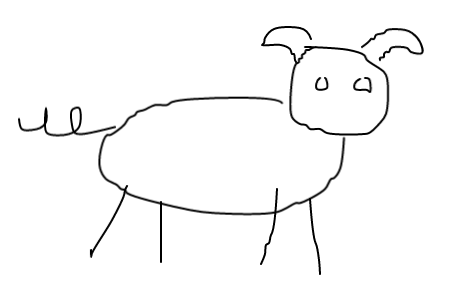
\includegraphics[scale=0.65]{malac.png}\\
Ha vége egy körnek, mert valaki ``malac''-ot kiáltott, akkor mindenki megszámolja, hogy az ő malaca mennyit ér. Minden testrész annyit ér, amennyit kellett dobni a lerajzolásához. A teljes malac 46 pont ($1+2+2*3+2*4+1*5+4*6$). A játékosok felírják a malacuk mellé a pontot és minden csoportból az adott körben legtöbb és legkevesebb pontot szerző játékosok felállnak és csoportot cserélnek, a legtöbbet szerző játékosok egy asztallal jobbra mennek a legkevesebbet szerzők egy asztallal balra mennek. Ha valamelyik asztalnál több legtöbb vagy legkevesebb pontot szerző játékos is van, akkor kő-papír-ollóval döntsék el, hogy ki marad és ki megy az asztaltól. Jöhet a következő kör. Akármennyi kört lehet játszani. Arra figyeljünk, hogy az első malac ne foglalja el az egész lapot. A végén össze lehet adni az összes pontot és egy végső nyertest hirdetni.

\item \textbf{Ninja:} A játék során az emberek megpróbálják a kezükkel lecsapni a másik játékos kézfejét és ezzel kiejteni, így a végén csak egy ember marad. A játék elején mindneki benyújtja középre a kezét, majd a játékvezető szavára mindenki egy-két nagy lépéssel hátralép és mozdulatlan marad. Ahogyan a benyújtott kezek közben sorban voltak a játékosok, úgy megyünk sorba. A kezdő játékos megpróbálja egy mozdulattal lecsapni egy bármelyik másik játékos kézfejét. Csak kézfejjel lehet lecsapni és csak kézfejre csapás ér (karórát, gyűrűt, \dots{} célszerű előtte levenni). A csapásnak egy mozdulatból kell állnia, azaz közben léphet előre/hátra, de célirányosan a másik kézfeje felé kell csapnia, ha támad. Lehet védekezőmozdulatot is csinálni (például ha az égbe emeljük mindkettő kezünket), de ennek is egy mozdulatnak kell lennie. Ha valamelyik játékos kézfejére próbál csapni a soros, akkor ő is tehet egy védekező mozdulatot, azaz elhúzhatja a kezét, de ennek is egy mozdulatnak kell lennie. A támadó játékos használhatja mindkettő kezét és így akár a másik játékos mindkettő kezét megcélozhatja. Ha talált, akkor az a játékos kiesik, akinek lecsapták a kezét. Ha nem talált, akkor ott kell hagynia a kezét, ahol lecsapta volna a másikét (tehát az szabálytalan, ha egy nagy karlendítéssel próbálom lecsapni a másik kezét és így irányzom, hogy a saját hónom alá kerüljön vissza a kezem, ha ő közben elhúzza az övét). Ezután a soron következő játékos jön; ez nem biztos, hogy ugyanaz, akit a mostani játékosunk támadott.

\item \textbf{Csoport számoljon el 20-ig:} Több (nagyjából) egyenlő létszámú csapat játssza, célszerűen legalább 5-6 fős egy csapat, de lehet akár 8-10 is. A játék célja, hogy a csapat elszámoljon 20-ig, az alábbi szabályokat betartva. Ha elrontják, akkor elölről kell kezdeniük.\\
Senki nem beszélhet vagy adhat ki hangot, csak ha számot mond. Egy számot csak egyszer lehet mondani. Mindig a soron következő számot kell mondani. Ha valaki mond egy számot, akkor a következőt nem mondhatja a mellette levő és ő maga sem. Nem lehet olyan mozdulatot tenni, vagy kommunikálni, ami a játék kimenetét befolyásolja (nem lehet mutogatni; nem lehet erősen valakire nézni, jelezve, hogy most ő jön; nem lehet kopogni vagy a másikhoz érni).\\
nincs meghatározva, hogy ki kezdi a játékot. A játékvezetőnek célszerű körbejárni a csapatok között, és ha hibát lát, akkor szólni, hogy kezdjék újra.

\item \textbf{Hagyd ki a hármast:} Körben kell lennie a játékosoknak és kijelölünk egy embert, aki kezdi a játékot, utána körben megyünk. 1-től kell mondani a számokat úgy, hogy ami hárommal osztható vagy amiben van 3-as, azt ki kell hagyni. (3,6,9,12,13,15,18,21,23,24,27,30,31,32, ... ) Akinek kéne mondani azt a számot, amit szabály szerint nem lehet kimondani, annak hallgatnia kell és az utána következőnek kell mondania. (tehát a harmadik embernek nem 4-et kell mondania, hanem hallgat és a negyedik ember mondja a 4-et). Ha valaki elrontja, az kiesik. Ha több egymást követő szám van, amit ki kell hagyni, akkor több ember marad ki.

\item \textbf{Kikötözött ceruzával rajzolj valamit:} 3-6 fős csapatokban játsszuk. Előkészületnél egy-egy filctollra/ceruzára kötözünk cérnát vagy spárgát, úgy hogy ki lehessen függőlegesen feszíteni, ha több ember fogja a zsineg végét. Társaságtól függően 20 cm-től 1 m-ig is lehet a zsineg hossza. Olyan íróeszközt kell választani, ami már akkor is fog, ha csak a saját súlya nyomja le. A játék elején meg kell határozni, hogy mit kell lerajzolni a csapatnak (lehet egy kivetített kép és le kell másolni, de lehet csak annyit mondani, hogy rajzoljanak egy autót). Az íróeszközhöz célszerű két pontot, alul és felül legalább 3-3 zsineget rögzíteni.

\item \textbf{Rúgd fel a cipőt az asztalra:} több csapatban is játszható. Egy asztalt helyezünk a játékosoktól bizonyos távolságba (2-6 méter) és a cipőjeiket/papucsaikat fel kell rúgni az asztalra. Leveszik a lábukról és a lábfejük végét visszadugják annyira, hogy tudjanak lendíteni egyet rajta. Előre tisztázni kell, hogy számít-e ha már fent volt a cipő, de egy másik cipő lelökte. Adott idő alatt kell valamennyit felrúgni vagy adot mennyiséget kell.

\item \textbf{Hettyem-pitty:} Körben ülnek a játkosok. Egy embert beállítunk középre és bekötjük a szemét. (Ha olyan a társaság, akkor adjunk neki egy párnát is.) A bekötött szemű odamegy valakihez és beül az ölébe vagy térdére (ha kell, akkor a párnát tegye maga alá), majd azt mondja, hogy ``hettyem'', mire az akinek az ölébe ült, azt válaszolja, hogy ``pitty''. Ekkor a bekötött szemű tippelhet, hogy ki az, ha kitalálja, akkor helyet cserélnek. Ha nem, akkor próbálkozhat mégegyszer. Ha ekkor sem találja ki, akkor tovább kell mennie más emberhez. Lehet az újrapróbálást 3-ra vagy 4-re növelni, ha nagy a társaság vagy nehezen megy a kitalálás. Célszerű eltorzítani a hangunkat. 

\item \textbf{2 igaz, 1 hamis:} Mindenki mond magáról 2 igaz és egy hamis állítást és a többieknek ki kell találnia, hogy melyik a hamis. (Csapatépítő játék, nem feltétlen kell pontozni.)

\item \textbf{Mássz át az asztal alatt:} Egy asztalt felállítunk és a tetejéről indulva át kell mászni alatt és visszaérkezni a tetjére úgy, hogy közben semmivel nem érinthetjük a földet. Pár embernek le kell fogni az asztalt, hogy az ne boruljon fel.

\item \textbf{Bogozd ki a kézcsomót:} Körben állnak az emberek és becsukják a szemüket. A játékvezető szavára mindenki elindul befelé a két kezét a kör közepe felé nyújtva (mint a filmekben a zombik). Ha eléggé közel értünk egymáshoz, akkor megfogunk egy-egy kezet a jobb és bal kezünkkel. A játékvezető (aki szintén játszhat), ha már megfogott két kezet, akkor figyelje, hogy minden rendben van-e (nincs-e olyan hely, ahol három kéz fogja egymást; vagy segítse ha már csak két kéz keresgél és nem találják  egymást). Ezután kinyitja mindenki a szemét és ki kell bogozni a kézcsomót úgy, hogy nem engedhetjük el egymás kezét közben. (Van olyan, hogy nem lehet teljesen kibogozni, de ez csak a végén derül ki). Egymás alatt, fölött kell átbújni.

\item \textbf{Székkel lóverseny:} A teremben kijelölünk egy indulóvonalat és egy célvonalat vagy annyi tárgyat, ahány játékos van és azt kell megkerülni és visszajutni az indulóvonalra. A játékban minden versenyző (célszerű egyszerre csak 2-4 embernek versenyeznie) feltérdel egy székre, a szék háttámlája kell, hogy a pálya felé nézzen és a támlát kell fogni. A játék indítása után nem szabad lelépni a székről és nem szabad semmi mást megérinteni a széken kívül. A támlát megrántva ugrásszerűen lehet előrehaladni. Könnyen fel lehet borulni és sérülést szerezni, szóval csak óvatosan.

\item \textbf{Egymás nyakába a láb, százlábú:} Több csapat felsorakozik egymással párhuzamosan. Pókjárás pozícióba helyezkednek és a lábaikat az előttük levő nyakába/vállára teszik. A sor elején levő ember lába a földön van, mindenki másnak csak a keze (és induláskor a feneke). A játékvezető szavára el kell indulni és egy előre meghatározott távot megtenni. Ha valakinek leér a feneke az nem baj, de nem szakadhat szét a százlábú.

\item \textbf{Piramis:} 6 embernek kell alkotnia egy piramist úgy, ahogy a pompomlányok csinálják. Négykézláb van mind a 6 ember. Alul 3, majd 2, végül 1. Figyeljünk, hogy az alattunk levőnek ne a gerincére rakjuk a lábunk/térdünk. 

\item \textbf{Ujj-párbaj:} 2 ember párbajozik egymással. Lehet úgy, hogy az egész társaság játszik és amikor lemegy egy kör, akkor a nyertesek versenyeznek és a végén egy marad. A páros jobb kezeikkel kezet fognak, de nem a hivatalos kézfogáshoz hasonlóan, hanem mint a feketék. A mutatóujjukat kinyújtják. Amikor a játékvezető elindítja a játékot, akkor az a céljuk, hogy a mutatóujjukkal megérintsék a másikat. (A jobb alkar nem játszik.) Ha valamelyik játékosnak sikerül, az nyer.

\item \textbf{Húzd rá a másikat a székre:} Körben áll a társaság és megfogják egymás kezét. Középen van egy szék (ha van egy nagyobb könnyű tárgy, például egy üres szennyeskosár vagy kuka, az talán jobb). A játékosoknak az a célja, hogy egymást ráhúzzák a székre. Aki hozzáér a székhez, az kiesik és szűkül a kör. Az utolsó két ember nyer. Ha szétszakad valahol a kör, akkor a szakadás mindkét oldalán álló kiesik. Ha van rá lehetőség, akkor szerezzünk 50-60 cm-es köteleket és kössünk mindkét végére csomót; az így kapott 30-40 cm-es köteleket használjuk. A játékosok ezt fogják így ha szétszakad a kör, akkor aki elengedte a kötelet csak az esik ki és nem a szakadás mindkettő oldala. Figyeljünk rá, hogy egyik változatnál se rángassuk a mellettünk álló kezét vagy a kötelet.

\item \textbf{Babzsák férfi-női név:} Körben áll a társaság és egy babzsákot dobálunk egymás között. Minden dobásnak egyértelműen egy ember irányába kell mennie és a dobó személy a dobás pillanatában mond egy keresztnevet. Ha a név azonos nemű, mint akinek dobták, akkor nem kapja el (elhúzza magát előle és a babzsák a földer esik); ha másik nemű a mondott név, akkor el kell kapnia. Ha hibázik az elkapó (elkapja, de nem kellett volna vagy nem kapja el, de el kellett volna), akkor kiesik. Fontos, hogy amikor a dobó kezét elhagyja a babzsák, akkor már a teljes név ki legyen mondva. Mindenki által ismert neveket mondjunk. A babzsákot alulról lendítve kell dobni és nem a másikhoz hozzávágni.

\item \textbf{LE-FEL:} Körben ül vagy áll a társaság és mindenki a saját térdét nézi. A játékvezető azt mondja, hogy ``FEL'' és ilyenkor az összes játékos felemeli a fejét és valakinek a szemébe néz. Ha két játékos egymás szemébe néz, akkor ők nagy jajveszékelés közben kiesnek. Mindig ``FEL'' után kötelező valakire nézni, nem szabad a plafont vagy bármi mást megcélozni a tekintetünkkel. Az utolsó 1-2 ember nyer. Ha egy menet lemegy és kiesnek, akik egymásra néztek, akkor a játékvezető a ``LE'' szóval jelzi, hogy mindenki nézze a saját térdét és új menet következik.

\item \textbf{Ülj le, ha igaz rád az állítás:} Mindenki áll és felolvas egy állítást a játékvezető, akire igaz ez az állítás, annak le kell ülnie. Az állvamaradottak játszanak tovább. Az utolsónak marad vagy akik utoljára esnek ki, azok nyernek. Ha nagy a társaság, abban az esetben új kör indulhat, akkor is, ha még 5-10 -en is állnak, hogy a többiek addig ne unatkozzanak.
/állításokat sorolunk (pl.: szereti a palacsintát) és ha igaz valakire, akkor az üljön le, aki állva marad, az nyer/

\item \textbf{Ülj jobbra ha igaz rád az állítás:} Körben ülünk, a játékvezető felolvas egy állítást, akire igaz az eggyel jobba ül. Aztán újabb állítást olvas fel, ha igaz rád akkor jobbra ülsz (lehet valakinek az ölébe), de ha ül valaki az öledben akkor nem ülhetsz jobbra, még akkor sem, ha pont ő is feláll és arrébb ül. A játék elején jegyezze meg mindenki, hogy melyik székről indult és aki leghamarabb oda visszaér, az nyer (akkor is, ha ha valakinek az ölébe kerül vissza, aki ott ül).

\item \textbf{Rajzold le a pároddal:} Asztalnál állnak párokban, a pár egyik fele elöl a másik hátul. A hátsó az elötte álló hónalja alatt benyújtja a kezét és ceruzával megpróbálja lerajzolni azt, ami a táblára fel van rajzolva vagy ki lett vetítve.  A hátsó nem nézheti sem a rajzot, sem a kivetített ábrát. Az elöl alló mondja neki, hogy merre húzza a vonalat. Csak egyszerű instrukciókat lehet adni (``Rajzolt egy vízszintes vonalat.'', ``Most balra egy kis kört.'', \dots{}), nem lehet egyértelműen a célábrára utaló utasítást adni (pl.: ``Rajzolt egy házat.'') Ha tehetjük, akkor a hátsónak kössük be a szemét; ebben az esetben akár állhatnak egymás mellett is.

\item \textbf{Húzzuk fel magunkat:} Körben ülünk 4-6-an és benyújtjuk a kezünket középre. Megfogjuk egymás kezét és fel kell húznunk magunkat álló helyzetbe, de a talpunk nem mozoghat.

\item \textbf{Lepedőleeresztős névkitalálós:} Két csoportra osztjuk a társaságot. Kell két ember, aki nem játszik, ők fogják tartani a lepedőt, ami nem lehet átlátszó, de még áttetsző sem. A két csapat a mellmagasságban tartott lepedő két oldalán helyezkedik el és (hang nélkül) kiválasztanak egy-egy játékost, aki a lepedőhöz térdel. A többiek kicsit távolabb vannak, hogy egyértelmű legyen ki a kiválasztott. Az egyik lepedőtartó a játékvezető, aki ad egy jelet mire leeresztik a lepedőt és a két kiválasztott játéko meglátják egymást. Amelyikőjük hamarabb ki tudja mondani a másik nevét, az elrabolja a másikat és az ő csapatuk egy taggal bővül. Ha egyszerre hangzik el a két név, akkor helyet kell cserélniük. Előre tisztázni kell, hogy becenevet elég mondani vagy teljes keresztnév, esetleg teljes név számít csak. A csapat többi tagja nem segíthet.

\item \textbf{Lény:} Kell hozzá egy legalább hátom részre szedhető zseblámpa és egyház, aminek van jópár terme, szobája. Valamint teljes sötétség, tehát ha az ablakon beivilágít a hold az már sok. A játék leején kiválasztjuk, hogy ki lesz a lény. A játékvezető kiküldi az embereket (a lényt is) és elrejti a házban a zseblámpa darabjait; ne legyen túl könnyű helyen, de hozzáférhető/megtalálható legyen. A játékosoknak tudniuk kell, hogy hogy néznek ki a zseblámpa darabjai. A játékvezető ezután lekapcsolja alámpákat és szól a lénynek hogy bejöhet. A lény elrejtőzik a házban. Ezután bejönnek az emberek és elkezdik keresni a zseblámpa darabjait. A lény előbújik és elkezdi megfogdisni az embereket. Akit megfogott, az mozdulatlan kell, hogy maradjon. Ha valaki, akit még nem fogott meg a lény megérinti a mozdulatlan embert, az újra mozoghat (kereshet és ki is szabadíthat másokat). Ha mindenkit megfogott a lény, akkor ő nyert. Az emberek célja, hogy megtalálják a zseblámpa darabjait; összeszereljék azt és rávilágítsanak vele a lényre, ekkor az emberek nyernek.

\item \textbf{Kidobó:} Ki kell jelölni előre egy pályát (létszámtól függően) amin kívül van legalább még egy méter szabad hely. Célszerű a szabadban játszani. Minden játékos a pályán belül áll, a jatékvezető háttal bedobja a labdát (lehet két vagy több labdával is játszani). Dobni, csak a pályán kívülről lehet, tehát ha megfogtam a labdát, akkor ki kell mennem vele együtt a pályán kívülre és onnan dobhatok. (A legrövidebb úton kell kimenni.) Ha dobtam, akkor vissza kell jönni. Ha valakit eltaláltak, az leguggol ott ahol kidobták és próbál újra játékba kerülni. Ennek kétféle módja van, egyik ha elkap egy labdát és kidob valakit (neki nem kell kimennie, hanem ahol guggol, onnan dob). Másik módja, ha hozzáér valakihez, aki játékban van a pályán belül. Ekkor akit megfogott, az guggol le és ő újra szabad. Akinél labda van azt nem lehet megfogni (annak pedig kötelessége a legrövidebb úton és időn belül kimenni a pálya szélére dobni). Ha valaki, aki szabad a pályán belülről dob, akkor le kell guggolnia (ha eltalált valakit, az szabad marad). Ha valaki elkapja a labdát, amit felé dobtak, akkor a dobó leguggol (ha alapból guggolt, akkor úgy marad). A guggoló embereknek nem szabad mozogniuk, a talpuk egy helyben kell, hogy maradjon. Aki kimegy a pályáról, az is le kell, hogy guggoljon. Aki utolsónak szabad marad, az nyer.

\item \textbf{Csipesz:} Egész alkalom alatt megy a játék. Valakire rárakja a játékvezető a csipeszt (a ruhájára vagy a hajába) úgy, hogy az ne vegye észre. Amikor az illető megtalálja, akkor megpróbálja továbbadni úgy, hogy akire csipteti, az ne vegye észre. Ha az átadás pillanatában lebukik, akkor nála marad a csipesz. Akinél az alkalom végén van a csipsz, vesztett, lehet csináltatni vele valamit (például ő mosogat).

\item \textbf{Stop:} Egész alkalom alatt megy a játék. Mindenkinek van egy ``stop""-ja és azt rámondhatja az alkalom alatt bárkire, akinek emiatt mozdulatlanul kell maradnia egy percig. Előre szögezzük le, hogy milyen helyzetben lehet használni a ``stop''-okat, hogy véletlenül se rontsuk el az alkalom többi részét.

\item \textbf{Postás:} Körben állunk, egy valaki középen áll. A körben levők közül valaki a levélfeladó, ő küldi a levelet valakinek a körben. Ezt úgy teszi meg, hogy hangosan kimondja, hogy ki a címzett: ``Küldöm a levelemet Józsinak''. Ezután a tőle jobbra vagy balra álló kezét megszorítja (csak az egyiket). Annak tovább kell szorítania és így eljut a levél a címzetthez. A küldő "elküldtem"-mel kell hogy jelezze azt a pillanatot, amikor a mellette levő kezé szorítja. A címzett "megkaptam"-mal jelzi, ha megkapta. A középen álló megpróbálja kitalálni, hogy hol tart a szorítás; hármat tippelhet; emberre kell mutatni, nem kézre; ha a mutatott ember valamelyik oldalán volt a szorítás, akkor aki szorított, az megy be középre. Amikor elindul a levél, a középen álló a küldő szemébe néz, csak az elküldés pillanata után nézhet másfelé, különben nagyon egyszerű lenne. A játék elején meg kell határozni, hogy legalább mennyivel távolabbi embernek kell küldeni a levelet (legalább 4-5 célszerű egy 15+ társaságban), hogy legyen útja a levélnek.

\item \textbf{Rabszolgás:} A játékvezetőhöz a játék előtt egyesével odamennek az emberek és mondanak egy álnevet (ez lehet fogalom, tárgy, név de mindenki által ismert nem hosszú szó kell, hogy legyen), ami az övék lesz, úgy hogy azt a játékvezetőn kívül más ne hallja. A játékvezető felírja egy papírra, hogy ki milyen álnevet mondott (azt is, hogy ki mondta meg az álnevet is). Ha mindenkinek van álneve, akkor a társaság leül egy körbe és a játékvezető felolvassa az álneveket (csak az álneveket és nem olyan sorrendben, amilyen sorrendben mondták neki). Ha sok játékos van, akkor kétszer is felolvashatja, de a játék folyamán többször nem (kivéve, ha nagyon elakadunk vagy még nem ismeri a társaság a játékot). Ezután kezdődik a játék egy választott játékos tippel. Mond egy nevet a társaságból és egy álnevet, pl.: ``Józsi, szerintem te vagy a labda''. Ha Józsi a labda, akkor a tippelő mögé kell ülnie székestül és a rabszolgája lesz, ezután megint az jön, aki az előbb volt. Ha nem találta el, akkor Józsi jön és ő tippel. Ha olyan embert találok ki, akinek már vannak rabszolgái, akkor tudnom kell, hogy nekik mi volt az álvenük (ez már egyszer ugye kiderült) és akkor őket is megszerzem, ha valaki álnevét nem tudom, akkor az kiszáll a játékból. Ha valakinek vannak rabszolgái, azoknak segíteniük kell a gazdájukat; ötletekkel, pl hogy milyen álnevek voltak még, amiket lehet mondani vagy pl ne azt tippelje, hogy ``Sanyi az áfonya'', mert azt már valaki mondta és nem talált. Aki a végén marad az nyer.

\item \textbf{Találd ki ki van rád írva:} Legalább annyi papírral kell előre készülni ahányan játszunk. Minden papírra a játékvezető előre felír egy híres személynevet vagy karaktert (pl.: Mózes, Jack Sparrow, Micimackó, ...). A játék elején mindenkinek a hátára ragasztunk egy nevet, amit ő nem lát. Amikor elindul a játék minden játékos megpróbálja kitalálni, hogy ki van a hátára írva. Ehhez eldöntendő kérdéseket kell feltenniük egymásnak; tehát odamegy az egyik játékos a másikhoz, megmutatja neki, hogy ki van a saját hátán és feltesz egy kérdést (pl.: Férfi vagyok?; Élő vagyok?; Meseszereplő vagyok?), mire a másik igennel vagy nemmel válaszol. Ekkor a másik is feltesz egy kérdést. Ha mindeketten válaszoltak, akkor mást kell keresniük. Egymás után nem lehet többet kérdezni ugyanattól az embertől, csak akkor lehet újra, ha már nincs olyan, akitől még nem kérdeztem. Aki először kitalálja, hogy ki ő az nyer.

\item \textbf{Hering/szardínia/:} Egy valaki elbújik a házban vagy udvaron, a többi elkezdi keresni, aki megtalálta, mellé bújik, az utolsónak megtaláló veszt és bújik el következőleg vagy ha van önként jelentkező, akkor ő.

\item \textbf{Egy forintos az állra:} Mindenki kap egy egyforintost vagy valamilyen hasonló apró tárgyat, de mindenki ugyanolyat kapjon. Feltesszük az állunkra (vagy a homlokunkra, de itt is legyen egység). Az indítás után lökdösni kell egymást a vállunkkal, csípőnkkel. Akinek leesik az egyforintosa, az kiesett. Miután elindult a játék nem szabad semmivel az egyforintoshoz érni vagy megigazítani. Figyeljünk egymásra, hogy ne okozzunk sérülést.

\item \textbf{Kacsintással rablás:} Körben állunk párosával, a pár egyik tagja a körben beljebb áll, mint a másik, aki mögötte áll és az elöl álló sarkát nézi. Egy ember egyedül van, ő rákacsint valamelyik elöl állóra, aki nem a szomszédja; akire kacsintott, az megpróbál odaszaladni hozzá, de a mögötte álló elkaphatja. Ha elkapta, akkor helyet cserél az elkapó és a szaladni vágyó, aki kacsintott egyedül marad és újra kacsint. Ha nem kapja el, akkor átmegy akire kacsintott, ahhoz aki kacsintott és beáll mögé. A hátul állóknak maguk mögött kell tartaniuk a kezüket. A hátul álló csak úgy kaphatja el az előtte levőt, hogy maximum az egyik lábával léphet el; ha mindkét lábával ellép az elkapáshoz, az nem érvényes és az elöl álló átmegy a kacsintó mögé.

\item \textbf{Komolyak és vidámak:} Alkossunk két csapatot, az egyiknek meg kell nevettetnie a másik minden tagját. Nézzük az időt, hogy meddig bírták, utána szerepcsere, és ezt az időt is lemérjük, aki tovább bírta, az a csapat nyer.

\item \textbf{Japán foci:} Körben állunk, terpeszve tett lábbal úgy, hogy összeérjenek a lábaink, tehát ne legyen rés a lábak között. Egy kisméretű labdát kel ütögetni a körön belül és akinek a lába között átmegy a labda, kiesett; ekkor szűkítjük a kört.A labdát csak ütni lehet, megfogni nem. A szomszédot nem lehet kiejteni (tehát az utolsó 3 ember nyer). A labdának a földön kell maradnia. Lehet azt csinálni, hogy aki térd fölé üti vagy magasan a körön kívülre, az kiesik.

\item \textbf{4 sarok:} Ha van lehetőség, használjunk ehhez a játékhoz kivetítőt. A játékvezető felolvas/kivetít egy kérdést és négy válaszlehetőséget, amiből csak az egyik helyes. A terem négy sarka jelöli a négy válaszlehetőséget (A, B, C, D sarok). Minden játékos beáll abba a sarokba amelyik válasz szerinte a helyes. Ha mindenki elhelyezkedett, a játékvezető elmondja a jó választ. Aki nem abban a sarokban állt, az kiesett. A maradék játékosnak szól a következő kérdés, az utolsónak maradó játékos nyer. Másik változatban, nincs kiesés; mindenki számolja, hogy mennyi helyes válasza volt és a végén a legtöbb helyesen válaszoló nyer.

\item \textbf{Válogasd szét:} 3-5 csapatban játsszuk, 3-8 fős legyen egy csapat. Mindegyik elé kiöntünk egy kupac keveréket (pl.: rizs és búza, vagy kukorica és bab) és szét kell válogatniuk minél előbb és pontosan. Ha valamelyik csapat elkészült, jelzi és a játékvezető ellenőrzi, hogy hibátlan-e. Ha pontos a szétválogatás, akkor nyert a csapat; ha van benne hiba, akkor a következőnek jelző csapaté az esély. Lehet úgy is játszani, hogy mérjük az időt, onnantól, hogy az első caspat jelzi, hogy végeztek és minden hibájukért valamennyi időlevonás jár (pl minden rossz kupacban levő búza/rizs +1 perc). Ha így is a többi csapat előtt végeznek, akkor nyertek. Természetesen a többi csapat kupacait is ellenőrizni kell.

\item \textbf{Kevés kéz és láb:} Megadott számú kéz és láb lehet csak lent a földön (pl. 15 embernél, 7 láb és 5 kéz). Olyan módon kell egymásra mászni, összekapaszkodni, hogy az előírt kéz- és lábszám teljesüljön.

\item \textbf{Bekötött szemű embert vezetni kell:} Kell egy vagy több akadálypálya és a bekötött szemű embert vezetik a többiek. Csak beszélni lehet hozzá, nem lehet hozzáérni. Egyszerre játszhatja több csapat is és nézzük, hogy kinek sikerül előbb visszaérnie. Lehet úgy is játszani, hogy csak egy ember beszélhet egy csapatból. Van olyan változat is, hogy a pálya szélén kell maradnia a beszéddel irányító embernek/csapatnak.

\item \textbf{Crebs soccer:} 4 csapat pókjárásba áll egy négyzet 4 oldala mentén. Mindenkinek van egy száma csapatonként, tehát például mindegyik csapat 1-től 10-ig be van számozva, középen van egy labda. A játékvezető mondd egy számot, akiké a szám, azok bemennek pókjárásba és megpróbálják a labdát kirúgni valamely másik csapat fölött. Amelyik csapat fölött kimegy a labda, az mínusz egy pontot kap. Jöhet a következő kör. Figyelni kell egymásra. Ki is lehet kötni, hogy nem szabad a másikhoz érni.

\item \textbf{Jelelős:} Mindenkinek van egy saját jele, ami egy mozdulat (pl. orrvakarás; erőltetett, széles mosoly; levegőbe rúgás). Egy ember áll középen, valaki (akiről nem tudja a középső, hogy ő az) kezdi a jelküldést, valaki más jelét mutatja és az az ember a saját jelével fogadja, ugyanígy azután akihez ment az küldi tovább; a középső tippelhet időközönként, hogy hol a jel (ne sűrűn, hogy ne legyen lelőve a lényeg). Addig nálam van a jel, amíg a másik el nem fogadta a saját jelével./

\item \textbf{Amerikából jöttem:} A kiválasztott pár közös megbeszélésük alapján valamilyen foglalkozást mutogat el. A többieknek pedig ki kell találni mi is az a foglalkozás. Ha kitalálták, cserélnek. A mutogatók természetesen nem beszélhetnek játék közben. A játék elején, amikor bejön a terembe a pár, azt mondják, hogy ``Amerikából jöttünk, mesterségünk címere: V-Ő''. A mesterség címere a foglalkozás első és utolsó betűje, például villanyszerelő esetén V-Ő. Amikor valki kitalálta, akkor a pár tagjai megkérdezik, hogy ``Kit választasz, cicát vagy kutyát?''. Ezt is előre meg kell beszélniük, hogy a melyikőjük a cica és melyikőjük a kutya. A kitaláló amelyiket választja, azzal megy ki a következő körre. A másik beül a játékosok közé. Lehet cica és kutya helyett akármi más.













\item \textbf{Faroklopás:} /Két csapat vagy játszható csapatok nélkül is, mindenkinek van egy darab rongy vagy kötél betűrve a nadrágjába. Cél kihúzni a másik nadrágjából a kendőt, akinek kihúzták kiesett./

\item \textbf{Piros lámpa, zöld lámpa:} /Egy ember áll a terep túloldalán. A többiek az ittenin. A túloldali háttal van az embereknek. A játék indulásakor mindenki elindul a túloldal felé, egyszer csak a túloldali visszafordul, ekkor mindenkinek mozdulatlanná kell dermednie. Ha valaki mozog az visszamegy a kezdőhelyre. Aki eléri a túloldalt, az cserél az ottanival. A túloldali többször is hátraéz és mindig visszaküldi a mozgókat.

\item \textbf{5 passzos:} /Két csapat, juttasd a labdát a kapushoz vagy a vödörbe, minimum 5 passz kell/

\item \textbf{Vidd a szádban a vizet:} és töltsd meg a vödröt

\item \textbf{Középen egy ember.:} Egy jelre mindenki elkezd énekelni valamit (hangosan) a középen álló találja ki, hogy melyik dalok ezek.

\item \textbf{Jobbkézrecsapós,:} Facepalm /Körben állunk, egy ember megy körbe belül, úgy hogy a kívül levő keze a szemét takarja (valahogy így http://i0.kym-cdn.com/photos/images/newsfeed/000/001/582/picard-facepalm.jpg?1240934151) a másikat ez a keze alatt kiteszi. Megy körbe, valak rácsap a kint levő kezére és ki kell találnia, hogy ki volt az, de csak a kör közepe felé fordulva fordulhat ki, hogy ránézzen az emberekre./

\item \textbf{"Szivi ha szeretsz, mosolyogj rám":} /Egy ember középen, odamegy valakihez ezt ~ mondja, ha az illető elmosolyodik/ elneveti magát, akkor helyet cserélnek; ha nem akkor megy tovább/

\item \textbf{Angol bulldog 1,2,3:} /Egy sáv van, abban áll egy ember, a többieknek át kell futniuk a sávon. Ha valakit elkap a középső, felemeli és kimondja, hogy "Angol bulldog 1,2,3" és eközben nem ejti le, akkor az az ember is bent marad a sávban. Előbb-utóbb majdnem mindenki bent lesz. Aki utolsó volt, az nyert./

\item \textbf{Kanapé:}

\item \textbf{Cápás:} /újságpapírdarabokra kell állni/

\item \textbf{Egymás hátára rajzolós:} /van két vagy több csapat, csapatonként sorbaállunk (egymás hátá nézzük), mindenki kap egy papírt és csapatonént egy-egy filc megy majd végig, a játék elején a vezető a hátul állok hátára tesz egy papírt és rajzol rá valami egyszerűt, ezután akin rajzolt az rajzol a papírjára úgy hogy az előtte állónak a hátára teszi; azt rajzolja le, amit érzett, hogy rá rajzoltak, végül az első is lerajzolja amit érzett és akié a legjobban hasonlót, az nyert/

\item \textbf{Állathangos párosítós:} /páros létszám szükséges, állatneveket osztunk ki emberneknek, egy fajtát két embernek, mindenki csak a sajátját tudja, egy jelre mindenki elkezdi a saját állatjának a hangját adni és párokba kell rendeződni/

\item \textbf{Húzd át a királyt a túloldalra:} /Két csapat, 3 részre osztott pálya, egy középső nagy rész és két oldalsó kisebb sáv; mindkét csapat választ egy királyt maguktól, de ezt csak ők tudják. A cél, hogy játékindítás után a saját szélső sávunkba behúzzuk, bevigyük a másik csapat királyát, ezt úgy csináljuk, hogy random emberkéket behuzigálunk, közben persze ők is visznek minket, a királyt lehet védeni de nem jó a feltűnés, mert akkor tudják kit kell bevinni, amelyik csapatnak sikerült az nyert/

\item \textbf{Kézre X:} /van egy vadász, aki az emberek kezére x-et rajzol, akinek rajzolt az kiesett, egész alkalmas játék, aki kitalálta hogy ki a vadász az tippelhet a játékvezetőnél, ha rossz a tipp, ő is kiesik és az is akire tippelt/

\item \textbf{Számháború:}

\item \textbf{Tölts és lőj:} /Tölteni, védekezni és lőni kell ütemre/

\item \textbf{Kanala:}s /Körben ülünk mindenkinél van 4 lap, az elsőnél a paklimaradék letéve, ő felhúz egy lapot és az így nála levő 5ből lerak egyet, ezt felhúzza a következő és ő is lerak egyet, közben az első már újat húzott, lényeg, hogy összejöjjön valakinél 4 darab ugyanolyan (mondjuk 4db  5-ös), ekkor a középen levő kanalakból az felkap egyet, mire mindenki megpróbál felkapni egyet. Középen eggyel kevesebb kanál van mint ahányan játszanak, így egy embernek nem jut, ő kiesik és vele együtt egy kanál is/

\item \textbf{Jelenet:} /4-6 önként jelentkező, egy bent marad, a többi kimegy, a bentinek elmondunk egy sztorit, behívunk egy embert, aki megfigyeli, ahogy a bent lévő elmutogatja a jelenetet, ő a következő behívottnak elmondja, hogy mit látott, ő megint mutogat, következő beszél ... az utolsó elmondja, hogy mi lehetett az eredeti sztori/

\item \textbf{Egy mondat körbesúgása:} /a poén, hogy mi sül ki belőle/

\item \textbf{Aláírásgyűjtés:} /A játék előtt (pár nappal, héttel) kell mindenkitől kérni egy dolgot, ami vele történt, rá igaz; de a többiek nem tudják. Ezeket kinyomtatni lapokra. A játék során mindenki kap egy ilyen lapot és egy tollat és odamennek egymáshoz és megkérdezik, hogy pl.: Te vagy aki már vezetett traktort?; ha igen akkor aláírja, ha nem akkor megy tovább és mástól kérdez, egy embertől egyszerre egyet lehet kérdezni, utána tovább kell állni. Lehet valami többekre igaz, akkor előfordulhat, hogy valaki lapján X, valakién pedig Y írta alá ezt a rubrikát/

\item \textbf{Rakd ki a szót:} /több csapat mindegyiknek kap 10-15 betűt (amilyen betűket kap egy csapat, olyanokat kap a másik is), a játékvezető körülír egy szót és ki kell azt találni, majd kirakni, amelyik csapat a leggyorsabb az kap pontot, jöhet a következő szó/

\item \textbf{Találd ki ki írta:} /Mindenki kap egy papírt, tollat és 5 percet, hogy írjon 4 szót, kifejezést, ami hozzá kapcsolódik, de nem egyértelmű (valamint a nevét, hogy tudja a játékvezető), ezután összeszedjük a papírokat, a játékvezeő felolvassa az első papírt és ki kell találni ki írhatta, aztán a követezőt; a nevetés a lényeg, nem a pontszerzés/

\item \textbf{Értelmező szótár:} /Hozunk egy értelmező szótárat vagy régi szavak gyűjteményét, keresünk olyan szavakat, amit nem ismernek az emberek, felolvasunk egyet és mindenki a kapott cetlijére leírja, hogy szerinte mi lehet az, a játékvezető leírja a helyeset is egy papírra, ezután összeszedjük a papírokat és felolvassuk mindet, közben az emberek tippelhetnek, hogy szerintük melyik az igaz (egy ember egyre szavazhat csak). Aki eltalálta hogy melyik a jó (ez csak akkor derül ki, ha mindet felolvastuk), az kap két pontot és akiére tippeltek az kap annyi pontot ahányan szavaztak rá/

\item \textbf{Csokivadászat:} /kör közepén 5-6 különböző csoki és/vagy édesség, megy körbe néhány dobókockapár, ha valaki duplát dob és tudja az egyik kaja nevét, akkor azt magához veheti, ha elfogyott középről vagy azt akarom ami másnál van, akkor azt úgy tudom megszerezni, hogy ha tudom a kaja nevét és annak a teljes nevét, akinél van; ha nem tudom senkijét/semmiét akkor nem szerzek semmit; egy ember több nyalánkságot is összeszedhet/

\item \textbf{Néma sor:} /mindenki kap egy számot, amit csak ő tud (n ember esetén 1-től n-ig osztjuk ki a számokat), a játék során sorba kell állni növekvő (csökkenő) sorrendben úgy hogy nem lehet közben beszélni és mutatni sem hogy hányas a tiéd/

\item \textbf{Faggass az ABC-vel:} /Mindenki kap egy papírt, amin az ABC betűi szerepelnek és körbe kelle menni kérdezgetni embereket és megtudni róluk dolgokat, amiket a kezdőbetűk segítségével egy-egy betű mellé fel tudsz írni. Egyszerre csak egyet kérdezhetsz egy embertől. Aki először ír minden betűhöz, az nyer. Pl.: "Milyen háziállatod van?" - "Kutya" - És akkor felírhatom, hogy XY-nak van egy kutyája, a "K" betűhöz./

\item \textbf{Név Roulette:} /Két egymást érintő körben kell felállni, mindenki a köre közepe felé fordul. Az érintés pontot meg kell jelölni valamivel (pohár, kislabda, szék, akármivel). Elindul a zene, elkezdenek a körök forogni. Amikor a zene megáll, akkor akik az érintési pontnál vannak megfordulnak és aki előbb mondja a másik nevét, az nyer, a vesztes átmegy a másik körbe. Addig tart, amíg az egyik kör el nem fogy, vagy le nem fújják a játékot./

\item \textbf{5 perc alatt 30 másodperces reklám:} /5 percet kapnak a csapatok, hogy egy megadott dologhoz reklámot készítsenek. Kell készülni előre tulajdonságokkal, amik az eladandó állatra/dologra jellemzőek és ezt a csapatoknak odaadni/kivetíteni. Ezt a reklámot elő is kell adni./

\item \textbf{Evőversenyek:} /zabkása kézzel, erőspaprika, bébikaja, marshmallow, háztartási keksz, stb.../

\item \textbf{Babakaja roulette:} /Körben ülünk és egy labda/bomba/akármi megy körbe. Akkor adhatod tovább, ha helyesen tudtál válaszolni a kérdésre, ha nem, akkor új kérdést kapsz. Akinél felrobban a bomba (tik-tak-bumm-ból mondjuk (lehet hogy túl rövid az)), vagy lejár az idő, az kell, hogy egy kanál bébiételt megegyen. (vagy akármit akármekkora előre megszabott mennyiségben). Sok kérdéssel kell készülni, amik többnyire kitalálhatóak/tudhatóak./

\item \textbf{Kulcsszavak:} /Az első embernek felolvas a játékvezető egy történetet, majd az elmeséli a másodiknak, az a harmadiknak és az a negyediknek. A negyedik pedig hangosan elmondja a történetet. Az elején meg kell jelölni 10 szót a sztoriban és ahány azok közül elhangzik az utolsótól, annyi pontot kapnak. (mindig csak az jön be, aki hallgatni fogja a sztorit és mindenki csak egyszer hallja)/

\item \textbf{Jelszó:} /Két pár versenyez. Mindkettőből egy-egy megkapja a szót. Rá kell vezetni a társad, hogy kitalálja mi az a szó. Egyszerre csak 1 szót mondhatsz rávezetésként, a társadnak az alapján kell kitalálnia. Ha nem sikerül, akkor a másik csapat jön, akiknek ugyanúgy egy szót szabad mondaniuk, de ők az előző csapat szavát is hozzávehetik. Így jönnek felváltva, amíg valamelyik csapatban ki nem találják a jelszót./

\item \textbf{Rabszolgamunka:} / http://www.ultimatecampresource.com/site/camp-activity/slaves-of-job.html

\item \textbf{Te, Én, Bal, Jobb:} /Neves játék. Körben ül mindenki, egy (vagy lehet töb emberrel is) ember pedig középen áll. Odamegy valakihez, rámutat és azt mondja, hogy "én"/"te"/"bal"/"jobb" és az ülőnek ez alapján kell a középen álló/saját/tőle jobbra ülő/tőle balra ülő nevét mondania (a középen levő ember felől nézzük az irányokat). Annyi ideje van kimondani ezt, amíg a középen álló el nem számol 5-ig korrekt sebességgel. Ha nem sikerül, vagy elrontja, akkor helyet cserélnek./

\item \textbf{WC-papír bemutatkozás:} /Körben ülünk, mindenkihez odamész és megkérdezed hány WC-papír darabot szeretne. Letépsz neki a kívánt számút, majd amikor mindenki megkapta amennyit szeretett volna, akkor mindenkinek ahány darab van nála, annyi féle dolgot kell magáról mondania./

\item \textbf{Forgalmi dugó:} /Felsorakoznak egy sorba, középen van egy üres hely és mindenki az üres hely felé (középre) fordul. A feladat az, hogy a két oldal helyet cseréljen. A szabályok: nem lehet hátrafelé haladni; csak üres helyre mozoghatsz előre; nem "ugorhatod át" csapattársadat; egyszerre csak egy ember mozoghat; egy helyen csak egy ember állhat egyszerre./

\item \textbf{Zombi:} /amit ifitáborban Halásziban játszottunk/ Vannak zombik (emberek, akiknek úgy kell járni mint egy zombinak, üvöltöznek is közben) és nekik a céljuk, hogy megvédjenek egy területet (cél). Vannak normál emberek, nekik a céljuk, hogy bejussanak a célba, ekkor szereznek pontot (egy ember bejut az egy pont). Az emberek egy start zónából indulnak és be kell jutniuk a cél zónába (célszerűen egy kör), anélkül, hogy egy zombi megérintené őket; ha ez mégis megtörténik, akkor ott ahol vannak leülnek, leguggolnak. Ha beért valaki a célba, akkor van egy pont és mehet vissza a starthoz újraindulni. Cél, hogy x darab pont meglegyen (létszámtól függ) y idő alatt. Ezen felül vannak gyógyítók, őket külön meg kell jelölni (pl kendő a csuklóra), nekik a feladatuk, hogy ha egy embert elkaptak a zombik, akkor odamehetnek, kézenfogva visszavihetik a starthoz és akkor az ember újra indulhat. Egy gyógyító egyszerre több embert is vihet. A gyógyító ezenfelül védheti is az embereket a testével, de nem erőszakosan.

\item \textbf{Elnökös:} /szintén Halászi, ifitábor/ Van egy elnök és neki 5-8 testőre /létszámtól függően/, akiket magának választ. Vannak a bérgyilkosok (mindenki más de legalább 3szor annyi, mint a testőrök), akiknek az a feladata, hogy megöljék az elnököt, mielőtt az megtalálja a kincset. A játék elején a bérgyilkosok eldugják a kincset a pályán, hogy az elnök és az emberei ne tudják. Az elnöknek van egy háza, onnan indulnak a testőrök és az elnök. A bérgyilkosok nem mehetnek be a házba. A játék indítása után a kincshez nem nyúlhat már senki, csak az elnök. A testőrök ha megérintenek egy bérgyilkost, az kiesik; ugyanez visszafelé, de a testőröket csak úgy lehet kiejteni, ha hátulról fogod meg (pl a hátát vagy a vádliját). Ha az elnököt megérintik a bérgyilkosok akárhol, akkor vége a játéknak, az elnök nem ejthet ki bérgyilkost. Célszerű úgy játszani, hogy a testőrök először megkeresik a kincset és utána hozzák ki az elnököt körbefogva, hogy szerezze meg a kincset.

\item \textbf{10 másodperces bújócska:} / 30 másodperc volt elbújásra és 20 keresésre. Akit megtalált és kimondta a nevét a húnyó, az esett ki.

\item \textbf{Pohárlefújós:} / Egy asztalt le kell fedni eldobható műanyag poharakkal, majd egy lufit kap minden csapat. Amelyik csapat előbb lefújja a lufiba fújt levegővel az összes poharat, az nyer.
\item \textbf{Mentsd a széket!:} / Rendezzük a székeket egy nagy körbe. Valaki álljon a kör közepén, mindenki más széken üljön és legyen egy extra szék. (20 fő esetén 2, 30 fő esetén 3, stb.)

A játék célja, hogy a középen álló személy leüljön egy üres székre, az összes többi ülő személy pedig próbálja megakadályozni őt ebben. Ezt úgy tehetik, hogy eggyel jobbra vagy balra ülnek, mielőtt a középen álló ember odaül (nem lehet a körön keresztül szaladni például). Egy idő után a középső ember sikeresen leül és a mellette jobbra vagy balra ülő ember (amelyik lassú volt odaülni) áll fel középre.
\item \textbf{Ügyetlen Bowling:} / A játék célja, hogy minél bénább legyél bowlingban, vagyis minél kevesebb pontot érj el. A pályát mi asztalok oldalra fektetésével határoztuk meg, egy bowling pályát alakítva velük. A pálya szélességét úgy állítottuk fel, hogy a piramisba felállított 10 bábu mellett ne férjen el a labda. A játék célja, hogy minél kevesebb pontot gyűjtsünk, azaz minél kevesebb bábut döntsünk le. Ha valaki az összes bábut lelöki a gurításával, akkor 0 pontot kap érte (a legkevesebb elérhető pontszám).

\item \textbf{Hernyó verseny:} / A csapatok felsorakoznak a kijelölt vonal mögött. Minden csapat választ magának egy egy szótagú hívószót (vagy a csapatnévvel is játszható ez), majd mindenki megfogja az előtte levő vállát. Csak páros lábú szökkenéssel lehet előre haladni, de egyszerre csak egy ember ugorhat. Ez a gyakorlatban úgy néz ki, hogy az indításkor az első ember előre szökken (közben fogja az ő vállát a mögötte álló ember), majd utána a második, majd a harmadik és így tovább, amíg el nem érik az utolsó embert. Amikor az utolsó ember is szökkent, akkor előrekiáltja a hívószavukat és ezt hallva az első szökkenhet egyet ismét. Szóval mindenki meg kell, hogy várja az előtte levő szökkenését, hogy ő is haladhasson, az elsőnek pedig az utolsó jelez, amikor ő is szökkent már. Az a csapat nyer, akitől az utolsó ember először áthalad a kijelölt célvonalon.

\item \textbf{Ejtsd le a fedőt:} / Mindenki egy körben ül székeken, egy ember pedig középen áll egy edény fedőjével a kezében (mi kanállal játszottuk, az is bőven megfelelt a célnak; lényeg, hogy hangos legyen amikor leesik). Odamegy egy ellenkező neműhöz a körben és felhúzza, majd fogja az ő kezét. Akkor a felhúzott ember keres egy ellenkező neműt és húzza fel. Ez így folytatódik és hosszabbodik a sor, míg az első ember el nem ejti a fedőt. Amikor az felszólal, akkor mindenki aki állt megpróbál leülni. Aki állva marad, az felveszi a fedőt és új kör kezdődik.

\item \textbf{Beltéri röpi:} / A háló egy sor asztalból áll a termen keresztbe, amin székek vannak. A székek felváltva az egyik és a másik csapat felé néznek. A játékot strandlabdával kell játszani. Minden csapatnak 3 érintése van, de fejjel és lábbal akárhányszor beleérhetnek (mi lábbal sem engedtük a lámpákat megóvandó). A falak és minden teremben levő eszköz is a játéktér része, megpattanhat rajtuk a labda, de ha plafont ér az, akkor a másik csapaté a pont. Pontozás és szervák igény szerint (mi 11-es meccseket játszottunk, ahol 3 szerva után cseréltek szervát).

\item \textbf{Vak vadász:} / Kell egy önkéntes, aki a vadász lesz. Az ő szemét be kell kötni és kap egy medence nudlit (mi korábban már más játékhoz kettévágtunk jópárat, úgyhogy így nem túl hosszú darabbal tudtunk most játszani). A vadász feladata az, hogy megüsse a nudlival a többi játékost, akit eltalál az kiesik és lejön a pályáról. Az a játékos nyer, aki az utolsó életben maradva. Ki kell jelölni a játékterületet, hogy a vadász feladata ennyivel egyszerűbb legyen. Ahogy fogytak a játékosok, úgy nyomtuk össze a területet. A vadász 10-15 másodpercenként elkiálthatja magát, hogy “Marco” és akkor minden életben levő játékosnak vissza kell kiáltania, hogy “Polo”, így a vadász nem csak a sötétben tapogatózik.
\end{itemize}

Széken ülő kosárlabda.
Egyszerűsített rögbi.
Parti-e?
Elnök titkár jegyző
Tenyér a tenyérhez párbaj, nem lehet ellépni
Körben labdadobálás, ne kapja el a középső
egymásnak forgatott asztalok, labdával kiütős.
Videóból kérdés.
Két labda körbe érje utol az egyik a másikat


\end{document}